\documentclass[11pt,a4paper]{article}
\usepackage[a4paper,hmargin=1in,vmargin=1in]{geometry}
\usepackage{pgfplots}
\pgfplotsset{compat=1.17}

\usepackage[czech]{babel}
\usepackage[utf8]{inputenc}
\usepackage[T1]{fontenc}

\usepackage{stddoc}
\usepackage{lipsum}
\usepackage{subcaption}

\newcommand{\plus}{{\texttt{+}}}
\renewcommand{\Re}{\operatorname{Re}}
\renewcommand{\Im}{\operatorname{Im}}
\newcommand{\fourier}[3]{\mathcal{F}_{#1}\!\left[#2\right]\!\left(#3\right)}
\newcommand{\ifourier}[3]{\mathcal{F}^{-1}_{#1}\!\left[#2\right]\!\left(#3\right)}


\begin{document}

\pagenumbering{arabic}

% Header
\begin{center}
    {\LARGE\textbf{Laboratorní úloha č. 2}}\\[3mm]
    \begin{minipage}{0.4\textwidth}
        \begin{flushleft}
            \textsc{\today}
        \end{flushleft}
    \end{minipage}
    ~
    \begin{minipage}{0.4\textwidth}
        \begin{flushright}
            \textsc{Martin Šimák}
        \end{flushright}
    \end{minipage}
    \noindent\rule{14.5cm}{0.4pt}
\end{center}

\paragraph*{Téma} Měření mikrovlnných generátorů

Cílem této úlohy bylo seznámit se se základními parametry mikrovlnných generátorů jako je stabilita výkonu generovaného signálu, fázový šum či potlačení rušivých složek vznikajících na výstupních obvodech generátoru.

\subsection*{Úkoly měření}
\begin{enumerate}
    \item Stabilita výkonu generovaného signálu generátorem HP 86250D.
    \item Fázový šum generovaného signálu generátory HP 86250D a R\&S SMF 100A na frekvenci 1~GHz.
    \item Fázový šum generovaného signálu generátorem ELSY SG2000.
    \item IP2 a IP3 generátorů ELSY SG2000 a R\&S SMF 100A na frekvenci 1~GHz.
    \item Odstup rušivých složek signálu generátoru ELSY SG2000.
\end{enumerate}

\subsection*{Použité přístroje a komponenty}
\begin{itemize}
    \item Spektrální analyzátor Agilent E4440A (3~Hz až 26,5~GHz)
    \item Zásuvná jednotka generátoru HP 86250D (8~GHz až 12,4~GHz)
    \item Řídící jednotka HP8620C
    \item Generátor ELSY SG2000 (100~kHz až 2~GHz)
    \item Generátor R\&S SMF 100A (1~GHz až 43,5~GHz)
    \item Propojovací SMA kabel Mini-Circuits CBL-2FT-SMSM\plus
\end{itemize}

\subsection*{Popis měření}
Z hlediska zapojení se jednalo o jednoduchou úlohu -- ve všech úkolech byl měřený generátor propojen SMA kabelem ke spektrálnímu analyzátoru, z něhož jsme odečítali hodnoty. Během všech úloh byl do spektrálního analyzátoru nahrán soubor dat obsahující potřebné korekce pro kompenzaci vložného útlumu propojovacího SMA kabelu na různých frekvencích podle katalogového listu. Tyto korekce jsou též obsaženy v tabulce~\ref{table:cable-CBL2FTSMSM-insertion-loss}.

\begin{table}[!ht]
\begin{center}
\begin{tabular}{| c | c || c | c || c | c |}
    \hline
    $f$ [GHz] & IL [dB] & $f$ [GHz] & IL [dB] & $f$ [GHz] & IL [dB] \\
    \hline
    0,05 & 0,09 & 5 & 0,63 & 10 & 0,94 \\
    \hline
    1 & 0,3 & 6 & 0,71 & 12 & 1,03 \\
    \hline
    2 & 0,41 & 7 & 0,74 & 13 & 1,1 \\
    \hline
    3 & 0,5 & 8 & 0,81 & 15 & 1,19 \\
    \hline
    4 & 0,57 & 9 & 0,87 & 18 & 1,32 \\
    \hline
\end{tabular}
\caption{Hodnoty vložného útlumu propojovacího SMA kabelu CBL-2FT-SMSM\plus}
\label{table:cable-CBL2FTSMSM-insertion-loss}
\end{center}
\end{table}

% Task 1
\paragraph*{Stabilita výkonu HP 86250D} Pro měření stability výkonu generovaného signálu generátorem HP 86250D jsme nastavili na spektrálním analyzátoru referenční hodnotu výkonu na 10~dBm, šířku mezifrekvenčního filtru na 1~MHz, rozsah zobrazovaných frekvencí v rozsahu 7~GHz až 13~GHz a trackujeme signál pomocí markeru. Na generátoru jsme zvolili režim CW (Continous Wave) a výkon signálu nastavili tak, abychom na analyzátoru viděli spektrální čáru na hladině zhruba 0~dBm. Hodnoty naměřeného výkonu generovaného signálu s frekvencí jemně laděnou v rozsahu 8~GHz až 12~GHz pomocí režimu \emph{CW Vernier} jsou zaznamenány v tabulce~\ref{table:stability-HP}.

\begin{table}[!ht]
\begin{center}
\begin{tabular}{| l || c | c | c | c | c | c | c | c | c |}
    \hline
    $f$ [GHz] & 8 & 8,5 & 9 & 9,5 & 10 & 10,5 & 11 & 11,5 & 12 \\
    \hline
    $P_G$ [dBm] & 0 & -0,15 & -0,58 & -0,8 & -0,43 & -0,15 & -0,07 & 0,06 & -0,2 \\
    \hline
\end{tabular}
\caption{Hodnoty výkonu generátoru HP 86250D na různých frekvencích}
\label{table:stability-HP}
\end{center}
\end{table}

% Task 2
\paragraph*{Fázový šum generátorů HP 86250D a R\&S SMF 100A} Měření fázového šumu je možné pomocí k tomu určené aplikace na použitém spektrálním analyzátoru. V aplikaci jsme nastavili nosnou frekvenci 10~GHz, rozsah hledání nosné 10~MHz a trackování nosné, přičemž rozsah zobrazování fázového šumu byl zvolen od -30~dBc (výkon vztažený k výkonu nosné) s krokem mřížky po 15~dB a rozsah offsetů od nosné na 1~kHz až 10~MHz. Po skončení zobrazování zahájeného funkcí \emph{Log Plot} jsme pomocí markeru odečetli hodnoty fázového šumu pro oba generátory, které jsou zaneseny v tabulce~\ref{table:phase-noise-HP-and-RS}. Nastavení generátoru HP 86250D bylo až na změnu frekvence na 10~GHz ponecháno z předchozí úlohy. Generátor R\&S SMF 100A byl uveden do základního nastavení a následně mu byl doladěn výstupní výkon na 0~dBm. Frekvence byla ponechána na 10~GHz, což je součástí základního nastavení použitého generátoru.

\begin{table}[!ht]
\begin{center}
\begin{tabular}{| l || c | c | c | c | c |}
    \hline
    $f_{\mathrm{off}}$ [kHz] & 1 & 10 & 100 & 1000 & 10000 \\
    \hline
    $\mathcal L_{\mathrm{HP}}$ [dBc/Hz] & -34,5 & -92,93 & -116,18 & -139,4 & -149,18 \\
    \hline
    $\mathcal L_{\mathrm{R\&S}}$ [dBc/Hz] & -103,4 & -111,83 & -117,06 & -131,64 & -143,58 \\
    \hline
\end{tabular}
\caption{Hodnoty fázového šumu generátorů HP 86250D a R\&S SMF 100A}
\label{table:phase-noise-HP-and-RS}
\end{center}
\end{table}

% Task 3
\paragraph*{Fázový šum generátoru ELSY SG2000 na 1~GHz a 2~GHz} Postup a nastavení úlohy byly ponechány z předchozího měření, neboť se liší pouze v měřeném generátoru. Hodnoty pro oba generované signály jsou zaznamenány v tabulce~\ref{table:phase-noise-ELSY}.

\begin{table}[!ht]
\begin{center}
\begin{tabular}{| l || c | c | c | c | c |}
    \hline
    $f_{\mathrm{off}}$ [kHz] & 1 & 10 & 100 & 1000 & 10000 \\
    \hline
    $\mathcal L_{1\mathrm{GHz}}$ [dBc/Hz] & -81,4 & -93,56 & -116,26 & -136,78 & -140,3 \\
    \hline
    $\mathcal L_{2\mathrm{GHz}}$ [dBc/Hz] & -75,27 & -88,07 & -110,98 & -131,98 & -136,95 \\
    \hline
\end{tabular}
\caption{Hodnoty fázového šumu generátoru ELSY SG2000 na 1~GHz a 2~GHz}
\label{table:phase-noise-ELSY}
\end{center}
\end{table}

\subparagraph*{Úkol} Na základě znalosti blokového schématu generátoru zdůvodněte, čím je způsoben rozdíl mezi oběma závislostmi.

Jak je vidět z obrázku~\ref{fig:elsy-sg2000-connection-scheme}, frekvence generovaného signálu generátorem ELSY SG2000 je řízena přímou číslicovou syntézou, která ladí referenční frekvenci krystalu pro fázový závěs. Tato část obvodu je schopna generovat kvalitní signál ve frekvenčním rozsahu 0~GHz až 1~GHz a následné navýšení probíhá pomocí frekvenčního násobiče. Ideální násobič zhoršuje fázový šum o $20 \log(N)$, kde $N$ je násobící poměr. Pro náš případ $N=2$ je tato teoretická hodnota zhoršení zhruba 6~dB.

\begin{figure}[!ht]
\begin{center}
    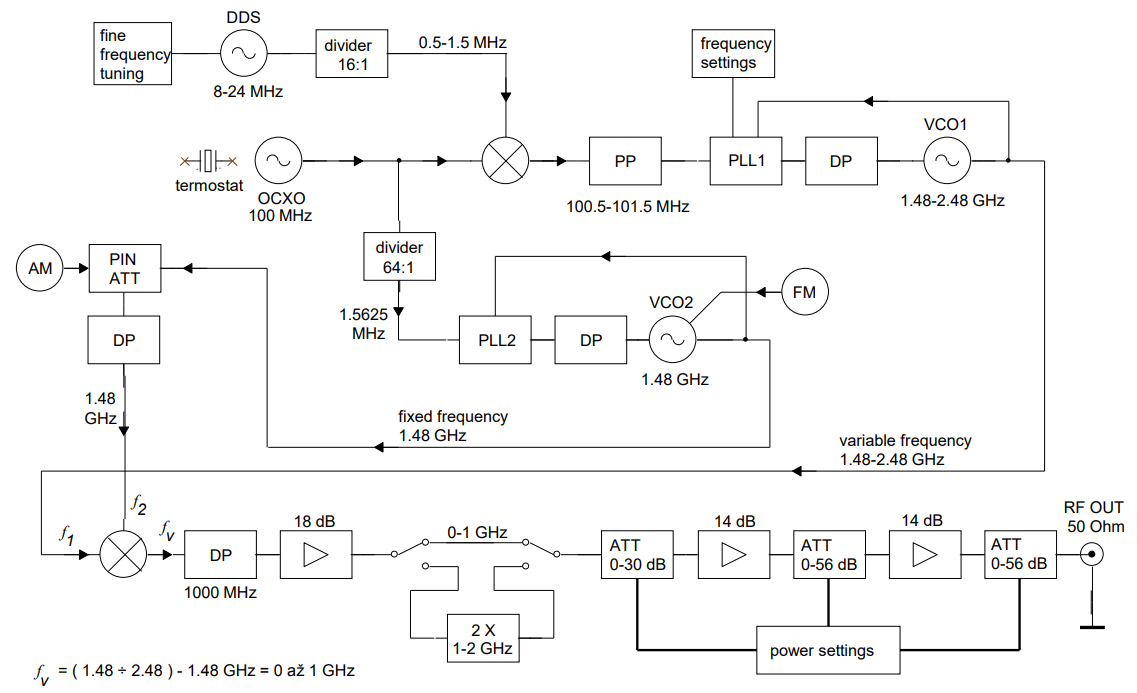
\includegraphics[width=0.8\textwidth]{src/elsy-sg2000_connection-scheme.png}
\end{center}
\caption{Blokové schéma zapojení generátoru ELSY SG2000}
\label{fig:elsy-sg2000-connection-scheme}
\end{figure}

% Task 4
\paragraph*{IP2 a IP3 generátorů ELSY SG2000 a R\&S SMF 100A} Pro měření intermodulačních produktů generátorů jsme resetovali nastavení spektrálního analyzátoru a nastavili jsme kromě korekce měřeného výkonu na použitý kabel rozsah frekvencí spektrálního analyzátoru na 100~MHz až 3,1~GHz, referenční výkon na 10~dBm a RBW na 20~kHz. Na frekvenci 1~GHz jsme následně měnili výkon generovaného signálu měřeným generátorem v rozsahu od prvního výskytu vyšších harmonických složek do 10~dBm. Hodnoty výkonu signálů na základní, 2. a 3. harmonické odečítané ze spektrálního analyzátoru pomocí markerů jsou zaneseny v tabulkách~\ref{table:intermodulation-products-ELSY}~a~\ref{table:intermodulation-products-RS} pro oba generátory. Na obrázcích~\ref{fig:elsy-sg2000-intermodulation}~a~\ref{fig:rs-smf-100a-intermodulation} jsou data vynesena graficky.

\begin{table}[!ht]
\begin{center}
\begin{tabular}{| l || c | c | c | c | c | c | c | c | c | c |}
    \hline
    $P_{\mathrm{set}}$ [dBm] & 10 & 6 & 2 & -2 & -6 & -10 & -14 & -18 & -22 & -26 \\
    \hline
    $P_{\mathrm{C}}$ [dBm] & 10,5 & 6,4 & 2,3 & -1,7 & -5,7 & -9,7 & -13,8 & -17,8 & -21,8 & -26 \\
    \hline
    $P_{\mathrm{IM2}}$ [dBm] & -21,2 & -31,8 & -42,4 & -47,7 & -51,7 & -64 & -68,4 & -72 & -76 & -78,6 \\
    \hline
    $P_{\mathrm{IM3}}$ [dBm] & -29,1 & -43,5 & -56,7 & -65,6 & -70 & -79 & -79 & -78 & X & X \\
    \hline
\end{tabular}
\caption{Hodnoty výkonů signálu na nosné frekvenci a intermodulačních produktů 2. a 3. řádu na výstupu generátoru ELSY SG2000}
\label{table:intermodulation-products-ELSY}
\end{center}
\end{table}

\begin{table}[!ht]
\begin{center}
\begin{tabular}{| l || c | c | c | c | c | c | c | c | c |}
    \hline
    $P_{\mathrm{set}}$ [dBm] & 10 & 5 & 0 & -5 & -10 & -15 & -20 & -25 & -30 \\
    \hline
    $P_{\mathrm{C}}$ [dBm] & 10,2 & 5,1 & 0,1 & -4,8 & -9,8 & -14,8 & -19,8 & -24,8 & -29,8 \\
    \hline
    $P_{\mathrm{IM2}}$ [dBm] & -30,3 & -40,7 & -50,8 & -51 & -61,3 & -60,9 & -70,6 & -70,9 & -77,5\\
    \hline
    $P_{\mathrm{IM3}}$ [dBm] & -55,1 & -69,8 & -77,3 & X & X & X & X & X & X \\
    \hline
\end{tabular}
\caption{Hodnoty výkonů signálu na nosné frekvenci a intermodulačních produktů 2. a 3. řádu na výstupu generátoru R\&S SMF 100A}
\label{table:intermodulation-products-RS}
\end{center}
\end{table}

\begin{figure}[!ht]
    \centering
\begin{subfigure}{0.45\textwidth}
    \centering
    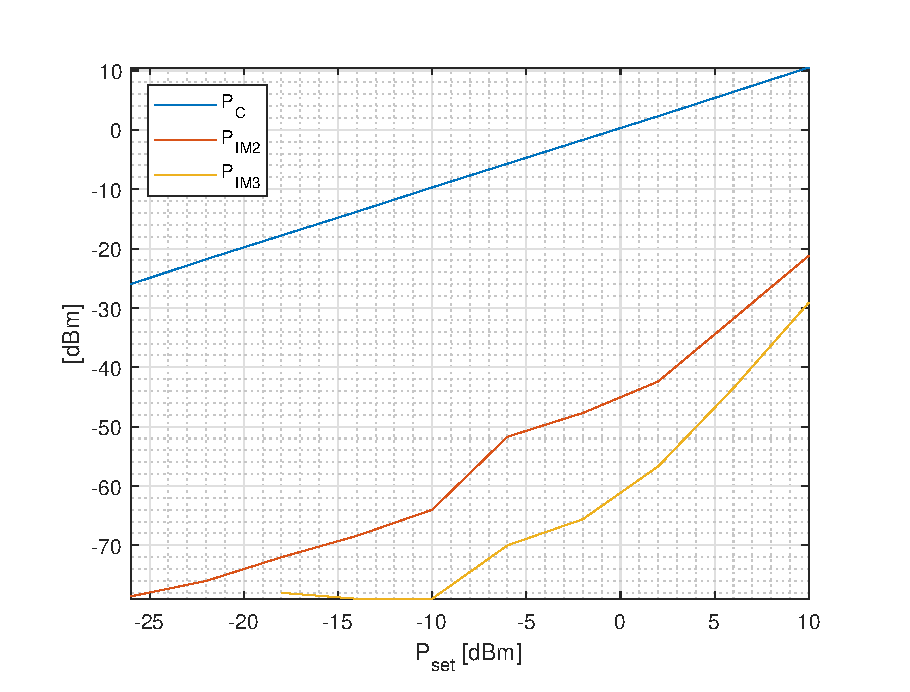
\includegraphics[width=\textwidth]{src/ELSY-SG2000-intermodulation.eps}
    \caption{ELSY SG2000}
    \label{fig:elsy-sg2000-intermodulation}
\end{subfigure}
\begin{subfigure}{0.45\textwidth}
    \centering
    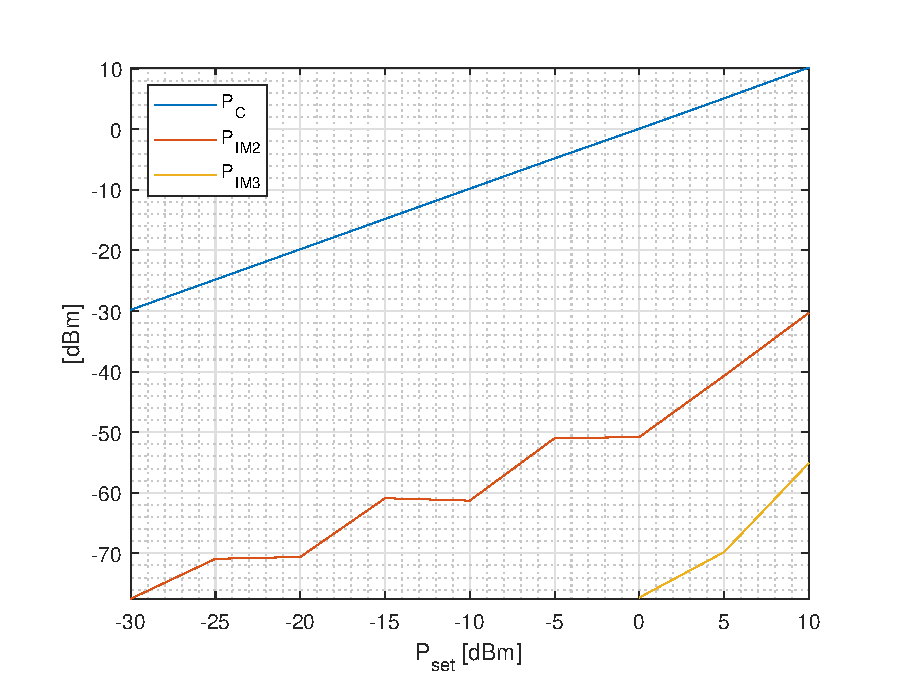
\includegraphics[width=\textwidth]{src/RS-SMF-100A-intermodulation.eps}
    \caption{R\&S SMF 100A}
    \label{fig:rs-smf-100a-intermodulation}
\end{subfigure}
\caption{Grafické zpracování dat pro ilustraci zahrazení IM2 a IM3}
\end{figure}

\subparagraph*{Úkol} Zjistěte hodnoty IP2 a IP3 pro oba měřené generátory.

V tabulce~\ref{table:intercept-points} jsou zaneseny body zahrazení získané pomocí aproximace lineárních tendencí intermodulačních produktů 2. a 3. řádu.
\begin{table}[!ht]
\begin{center}
\begin{tabular}{| l || c | c |}
    \hline
    & IP2 [dBm] & IP3 [dBm] \\
    \hline\hline
    ELSY SG2000 & 48,2 & 37,6 \\
    \hline
    R\&S SMF 100A & 48,6 & 32,5 \\
    \hline
\end{tabular}
\caption{Zjištěné hodnoty IP2 a IP3}
\label{table:intercept-points}
\end{center}
\end{table}

% Task 5
\paragraph*{Odstup rušivých složek signálu generátoru ELSY SG2000}
Pro zobrazování intermodulačních a subharmonických složek generovaného signálu jsme nastavili spektrálnímu analyzátoru rozsah na měření do 6,2~GHz a RBW na 100~kHz. Pomocí delta markeru jsme naměřili hodnoty odstupu nejvýznamější rušivé složky signálu od nosné v závislosti na výstupním výkonu generovaného signálu $P_{\mathrm{set}}$ o frekvenci 2~GHz. Tyto hodnoty jsou zaznamenány v tabulce~\ref{table:spurious-signal-distance-ELSY}.

\begin{table}[!ht]
\begin{center}
\begin{tabular}{| l || c | c | c | c | c | c | c | c | c |}
    \hline
    $P_{\mathrm{set}}$ [dBm] & 10 & 5 & 0 & -5 & -10 & -15 & -20 & -25 & -30 \\
    \hline
    $\Delta P$ [dBm] & -28,4 & -27 & -25,3 & -23,8 & -23,2 & -25,7 & -23,2 & -25 & -23,4 \\
    \hline
\end{tabular}
\caption{Odstup nejsilnějšího rušivého signálu od žádoucího na různých úrovních výkonu}
\label{table:spurious-signal-distance-ELSY}
\end{center}
\end{table}

\subparagraph*{Úkol} Na základě znalosti blokového schématu generátoru zdůvodněte změřenou závislost.

Závislost je nepravidelná vlivem toho, že nastavení výkonu je realizováno přímým laděním atenutárorů, kterými je regulován výkon přivedený na vstupy zesilovačů, jak je vidět na obrázku~\ref{fig:elsy-sg2000-connection-scheme}. Nelinearita operačních zesilovačů potom způsobuje nepravidelný odstup intermodulačních a subharmonických složek signálu generátoru.

\subsection*{Závěr}
V rámci úlohy jsme se seznámili s měřením základních parametrů mikrovlnných generátorů. Měření probíhalo tak, aby nám umožnilo porovnat kvalitu měřených generátorů, což posloužilo jako demonstrace odlišností jednotlivých konstrukcí. Mohli jsme tak například sledovat negativní dopad absence fázového závěsu na stabilitu výkonu generovaného signálu starším, \emph{napěťově syntetizovaným} generátorem HP 86250D či rozdíly ve schopnosti potlačení fázového šumu oproti vysoce kvalitnímu, \emph{frekvenčně syntetizovanému} generátoru R\&S SMF 100A.

Měření proběhlo v pořádku bez větších obtíží.


\end{document}
